\documentclass[UTF8, a4paper, 12pt]{ctexart}

% 基础包
\usepackage{amsmath}
\usepackage{amssymb}
\usepackage{enumitem}
\usepackage{booktabs}
\usepackage{tabularx}
\usepackage{graphicx}
\usepackage{geometry}
\usepackage{float}
\usepackage{hyperref}

% 代码高亮
\usepackage{listings}
\usepackage{xcolor}

% 页面设置
\geometry{
    left=2.5cm,
    right=2.5cm,
    top=2.5cm,
    bottom=2.5cm
}

% 代码样式设置
\lstset{
    basicstyle=\ttfamily\small,
    breaklines=true,
    showstringspaces=false,
    commentstyle=\color{gray},
    keywordstyle=\color{blue},
    stringstyle=\color{red},
    frame=single,
    numbers=left,
    numberstyle=\tiny\color{gray}
}

% 超链接设置
\hypersetup{
    colorlinks=true,
    linkcolor=blue,
    filecolor=magenta,      
    urlcolor=cyan,
    citecolor=green
}

\begin{document}


\section{LaTeX 兼容图片格式测试}


本文档测试 LaTeX 原生支持的图片格式。


\subsection{支持的图片格式}


\subsubsection{1. JPEG 格式图片}


JPEG 是 LaTeX 原生支持的格式,适合照片和复杂图像。


\begin{figure}[H]
    \centering
    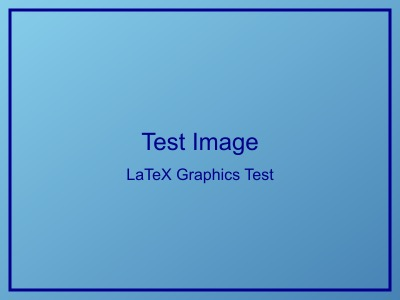
\includegraphics[width=0.8\textwidth]{../../tests/images/test_image.jpg}
    \caption{JPEG 测试图片}
    \label{fig:jpeg_____}
\end{figure}



\subsubsection{2. PNG 格式图片}


PNG 也是 LaTeX 原生支持的格式,支持透明度,适合图标和截图。


\begin{figure}[H]
    \centering
    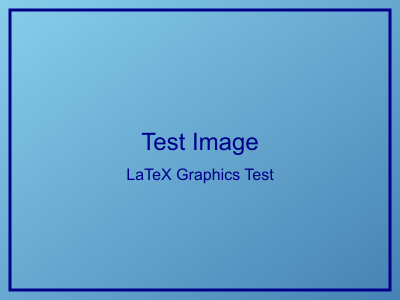
\includegraphics[width=0.8\textwidth]{../../tests/images/test_image.png}
    \caption{PNG 测试图片}
    \label{fig:png_____}
\end{figure}



\subsection{图片处理功能验证}


\subsubsection{路径解析测试}


上面的图片使用相对路径,测试路径自动修复功能:

\subsubsection{LaTeX 图片环境}


每个图片都应该生成完整的 figure 环境:


\begin{lstlisting}[language=TeX, basicstyle=\ttfamily\small, breaklines=true]
\begin{figure}[H]
    \centering
    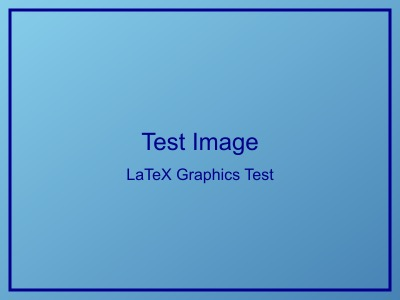
\includegraphics[width=0.8\textwidth]{../../tests/images/test_image.jpg}
    \caption{JPEG 测试图片}
    \label{fig:jpeg_测试图片}
\end{figure}

\end{lstlisting}


\subsection{预期结果}


\subsection{图片质量和性能}


\subsubsection{文件大小对比}


\subsubsection{显示效果}


两种格式都应该在 PDF 中正确显示,保持原始的颜色和清晰度。


\subsection{测试总结}


这个测试验证了:


\end{document}
